
\chapter{cpu\_serial.c, cpu\_serial.h}\label{ch:cpu_serial}

    The following code provides a serial interface to an FPGA. The FPGA code uses
    modules uart\_rx() and uart\_tx() in library uarts.3pl for serial
    transmission via the host computer port.
    
    The .info file for the design contains the read and write addresses,
    data types and bit counts and the interrupt numbers. This is all
    transfered to the associated .h file by python script uart\_info2c for
    inclusion in the CPU C source code.
    
    Each command from the CPU to the FPGA begins with the following byte
    
    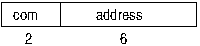
\includegraphics{comm}
    
    The two-bit command is -
    
    \begin{tabular}{ l  l }
        00   & read value, read queue \\
        10   & write static, write queue \\
        01   & read memory \\
        11   & write memory \\
    \end{tabular}
    
    The 6-bit address allows access 64 writable and 64 readable locations
    in the FPGA.
    
    For a write to a static or queue variable the format is -
    
    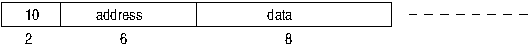
\includegraphics{commw}
    
    where the command is followed by zero or more data bytes (a zero-length
    write has no data but the write can act as a trigger or event).
    There is no response from the FPGA.
    
    For a read from a value or a queue the format is -
    
    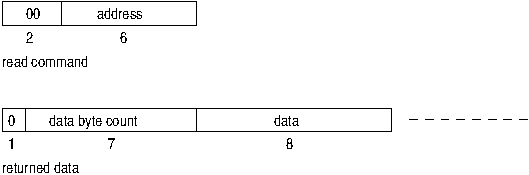
\includegraphics{commr}
    
    where the returned data consists of a data byte count and one or more data
    bytes.
    
    For a write to memory -
    
    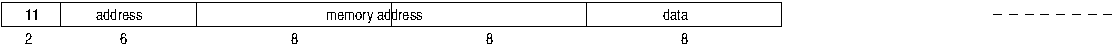
\includegraphics{commmw}
    
    where the command is followed by 16-bit memory address and one or more
    data bytes. There is no response from the FPGA.
    
    For a read from memory -
    
    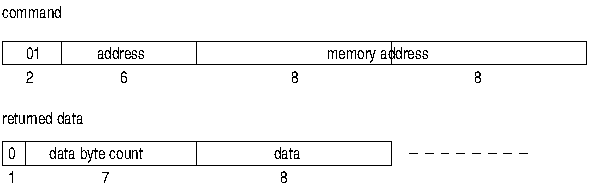
\includegraphics{commmr}
    
    where the command is followed by 16-bit memory address.
    A data byte count and one or more data bytes are returned from the FPGA.

    
    Interrupts are initiated by the FPGA unlike the previous transfers which
    are all initiated by the CPU.
    For an interrupt the FPGA sends a single byte to the CPU. The byte has
    the most significant bit set and the remaining 7 bits indicates the
    interrupt number.

    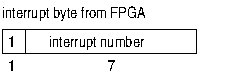
\includegraphics{commint}
    
    An interrupt byte will not be sent during the transmission of a CPU command
    and any associated return data or during a DMA transfer (see below).
    
    DMA requests by the FPGA code are of course carried out by software in
    the CPU (there being no hardware connection for real DMA) and are initiated
    by the FPGA.

    For DMA write from FPGA to CPU -
    
    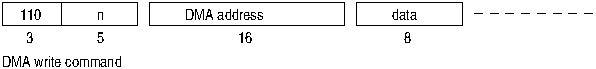
\includegraphics{commdmaw}
    
    For DMA read to FPGA from CPU -
    
    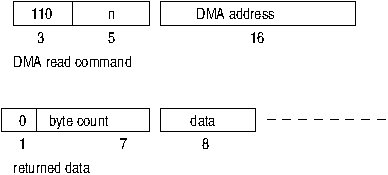
\includegraphics{commdmar}
    

        
    Commands and associated data are written to port file desriptor fd. Data
    received from the FPGA is read from {\bf fd} in the input handler which runs
    in its own thread. A received byte with the top bit set is an interrupt, the
    remaining bits giving the interrupt number (semaphore index). A sem\_post()
    is issued to the semaphore with that index. A received byte with the top bit
    clear is a byte count for data to be received from the FPGA. The following
    bytes indicated by the count are read from {\bf fd} and written to pipe {\bf
    pipefd[1]}. A command expecting received data waits on {\bf pipefd[0]} and
    reads from it (a command knows in advance how many bytes to expect as
    this is contained in the .info file).
    
    
    sem\_wait()
    
    \begin{lstlisting}[gobble=4, language=C]
        #include    "cpu_serial.h"

        #define BSIZE   1024

        sem_t**         sem;
        char**          sem_name;
        char            buffer[BSIZE];
        int             fd;
        struct termios  tio;
        static int      pipefd[2];
        pthread_t       tideh;
        int             ninterrupts;

        int         open_port (char* pname);
        void        close_port ();
        void        write_ (
                        char*   ptr,
                        int     bytes
                    );
        int         read_ (
                        char*   ptr,
                        int     bytes
                    );
        void*       input_handler ();

        void
        open_cpu_serial(char* pname, int interrupts) {
            ninterrupts = interrupts;
            fd = open_port(pname);
            pipe(pipefd);
            if (ninterrupts != 0) {
                sem = (sem_t**)malloc(ninterrupts * sizeof(sem_t*));
                sem_name = (char**)malloc(ninterrupts * sizeof(char*));
                for (int i=0 ; i<ninterrupts ; i++) {
                    sem_name[i] = (char*)malloc(6);
                    sprintf(sem_name[i], "/e%d", i);
                    sem_unlink(sem_name[i]);    // remove if already exists!
                    if ((sem[i] = sem_open(sem_name[i], O_CREAT, 0600, 0)) == SEM_FAILED) {
                        perror("sem_open");
                        exit(1);
                    }
                }
            }
            tideh = thread_start(input_handler, "input_handler", 1);
        }

        void
        close_cpu_serial() {
            pthread_cancel(tideh);
            for (int i=0 ; i<ninterrupts ; i++) {
                sem_close(sem[i]);
                sem_unlink(sem_name[i]);
            }
            close_port();
            close(pipefd[0]);
            close(pipefd[1]);
        }

        void
        comms_write (
            int         mem,        // memory write 1, static or queue write 0
            uint8_t     address,    // FPGA register address
            uint16_t    memaddress, // memory address if required
            int         bytes,      // number of data bytes
            char*       ptr         // pointer to data
        ) {
            char    com = 0x80 | (mem << 6) | address;
            int     i;
            int     n = bytes;

            write_(&com, 1); // send command byte
            if (mem != 0)
                write_((char*)&memaddress, 2); // send memory address
            while (n > 0) {
                i = write(fd, ptr, n);
                n -= i;
                ptr += i;
            }
        }

        void
        write_ (
            char*   ptr,
            int     bytes
        ) {
            int i;

            if (write(fd, ptr, bytes) < 0) {
                fprintf(stderr, "data write error\n");
                exit(1);
            }
        }

        void
        comms_read (
            int         mem,        // memory read 1, value or queue read 0
            uint8_t     address,    // FPGA register address
            uint16_t    memaddress, // memory address if required
            int         bytes,      // number of data bytes to be received
            int         sig,        // 1 if signed, 0 if unsigned
            int         fill,       // number of top bytes to fill
            char*       ptr         // pointer to data destination
        ) {
            char    com = (mem << 6) | address; // set address and memory flag in command
            int     n = bytes;  // byte counter initialisation
            char    snap;       // most significant byte
            char    pad = 0;    // padding byte - 0 or 0xff
            int     i;
            // send command byte
            write_(&com, 1);

            // send memory address if is a memory read
            if (mem != 0)
                write_((char*)&memaddress, 2);

            // receive data and write to destination address
            while (n > 0) {
                i = read_(ptr, n);
                n -= i;
                ptr += i;
            }
            snap = *(ptr - 1);

            // if whole result type has been filled, return
            if (fill == 0)
                return;

            // fill remainder of result with 0x00 (unsigned or +ve) or 0xff (signed and -ve)
            if ((sig != 0) && ((snap & 0x80) != 0))
                pad = 0xff;    // 0xff if signed and -ve
            while (fill-- != 0)
                *ptr++ = pad;   // fill most significant bytes
        }

        int
        read_ (
            char*   ptr,
            int     bytes
        ) {
            int r;
            r = read(pipefd[0], ptr, bytes);
            if (r < 0) {
                fprintf(stderr, "data read error\n");
                exit(1);
            }
            return(r);
        }

        void*
        input_handler () {
            int     r;
            char    c;
            int     n;
            int     bytes;
            char*   ptr;

            for (;;) {
                r = read(fd, &c, 1);
                if (r < 0) {
                    printf("uart read error\n");
                    exit(1);
                }
                n = c & 0x7f;   // byte count or interrupt ID
                if (c & 0x80) {
                    // is an interrupt
                    if (n >= 20)
                        printf("interrupt %d illegal (max 20) - ignored\n", n);
                    else
                        sem_post(sem[n]);
                } else {
                    // is a command return -
                    // read the data
                    bytes = n;
                    ptr = buffer;
                    while (bytes > 0) {
                        r = read(fd, ptr, bytes);
                        bytes -= r;
                        ptr += r;
                    }
                    // write the data back to the command requesting it
                    bytes = n;
                    ptr = buffer;
                    while (bytes > 0) {
                        r = write(pipefd[1], ptr, bytes);
                        bytes -= r;
                        ptr += r;
                    }
                }
            }
        }

        int
        open_port (char* pname) {
            int             fd;
            struct termios  ntio;
            int             flags;

            if (strlen(pname) == 0) {
                fprintf(stderr, "could not find USB serial device");
                exit(1);
            }

            fd = open(pname, O_RDWR | O_NOCTTY | O_NONBLOCK);
            if (fd < 0) {
                fprintf(stderr, "Cannot open USB serial device\n");
                exit(1);
            }
            printf("port %s open\n", pname);

            // Make the file descriptor blocking.
            flags = fcntl(fd, F_GETFL);
            flags &= ~O_NONBLOCK;
            fcntl(fd, F_SETFL, flags);


            tcgetattr(fd, &tio); // get current port settings
            bzero(&ntio,sizeof(ntio)); // clear struct for new port settings
            ntio.c_cflag = CS8 | CREAD | CSTOPB | CLOCAL;
            ntio.c_iflag = IGNPAR;
            ntio.c_oflag = 0;       // OCANON
            ntio.c_lflag = 0;       // ICANON
            ntio.c_cc[VMIN] = 1;    // blocking read until 1 character arrives
            ntio.c_cc[VSTART] = _POSIX_VDISABLE;
            ntio.c_cc[VSTOP] = _POSIX_VDISABLE;
            ntio.c_cc[VINTR] = _POSIX_VDISABLE;
            ntio.c_cc[VQUIT] = _POSIX_VDISABLE;
            ntio.c_cc[VSUSP] = _POSIX_VDISABLE;
            cfsetispeed(&ntio, B115200);
            cfsetospeed(&ntio, B115200);

            tcflush(fd, TCIFLUSH);
            tcsetattr(fd, TCSANOW, &ntio);

            return(fd);
        }

        void
        close_port () {
            // Restore terminal settings
            tcsetattr(fd, TCSANOW, &tio);
            close(fd);
        }

        // Start a thread.
        pthread_t
        thread_start(
            void *  (*func)(void*),
            char *  name,
            int     priority
        ) {
            int                 status;
            struct sched_param  sp;
            pthread_t           tid;

            if ((status = pthread_create(&tid, NULL, func, NULL)) != 0) {
	        printf("thread_start(): pthread_create() failed thread '%s' (err = %s)\n",
	            name, strerror(status));
                exit(1);
            }

            sp.sched_priority = priority;

            status = pthread_setschedparam(tid, SCHED_RR, &sp);
            if (status != 0) {
    	        printf("thread_start(): pthread_setschedparam() failed for thread '%s' (err = %s)\n",
	            name, strerror(status));
                exit(1);
            }
            return(tid);
        }
    \end{lstlisting}
    


\chapter{cpu\_serial.py}

    The Python3 version of this code functions the same way as the
    C version above -

    \begin{lstlisting}[gobble=4, language=Python]
        import os
        import fcntl
        import termios
        import queue
        import threading

        tio = None
        infile = None
        fd = None
        q = queue.Queue()

        # Write data to FPGA.
        #   mem         0 if static or queue write, 1 if memory write
        #   address     FPGA interface address
        #   memaddress  memory address if mem == 1
        #   dba         byte array of data to send
        #
        def comms_write (mem, address, memaddress, dba):
            ba = bytearray()
            ba += bytes([0x80 | (mem << 6) | address])          # command
            if mem != 0:
                ba += memaddress.to_bytes(2, byteorder='little')# append memory address
            if dba != None:
                ba += dba                                       # append data
            os.write(fd, ba)                                    # write to FPGA

        # Read data from FPGA.
        #   mem         0 if value or queue read, 1 if memory read
        #   address     FPGA interface address
        #   memaddress  memory address if mem == 1
        #   bytes       data length - NOT USED HERE (required by Zynq)!
        #
        def comms_read (mem, address, memaddress, bytecount):
            global q
            wba = bytearray()
            wba += bytes([(mem << 6) | address])                # command - address and memory flag
            if mem != 0:
                wba += memaddress.to_bytes(2, byteorder='little')# append memory address
            os.write(fd, wba)                                   # write to FPGA
            return(q.get())                                     # read response from FPGA


        # Close the serial port to the FPGA.
        def close_port ():
            # Restore terminal settings
            tcsetattr(fd, TCSANOW, tio)
            close(fd)

        # Handle input from FPGA via serial port.
        def input_handler ():
            global fd
            global q
            while True:
                try:
                    r = os.read(fd, 1)
                except OSError:
                    print("UART read error")
                    exit(1)
                c = r[0]
                n = c & 0x7f    # Note: max of 127 bytes
                if c & 0x80:
                    # is an interrupt
                    if n >= 20:
                        print("interrupt " + str(n) + " illegal (max 19)")
                        exit(1)
                    else:
                        semaphores[n].release()
                else:
                    # is a command return - read the data            
                    buff = bytearray()
                    while n > 0:
                        buff += bytes(os.read(fd, n))
                        n -= len(buff)
                    q.put(buff)

        # Open the serial port to the FPGA.
        def open_cpu_serial (pname, ninterrupts):
            global fd
            global tio
            global semaphores

            if len(pname) == 0:
                print("could not find USB serial device" + pname)
                exit(1)
            try:
                # Open initially as non-blocking so it does not wait trying to read
                # as it is opened.
                fd = os.open(pname, os.O_RDWR | os.O_NOCTTY | os.O_NONBLOCK)
            except OSError:
                print("Cannot open USB serial device")
                exit(1)

            # Having opened the file and continued, now make the file
            # descriptor blocking.
            flags = fcntl.fcntl(fd, fcntl.F_GETFL)
            flags &= ~os.O_NONBLOCK
            fcntl.fcntl(fd, fcntl.F_SETFL, flags)

            tio = termios.tcgetattr(fd) # get current port settings
            ntio = termios.tcgetattr(fd)

            ntio[0] = termios.IGNPAR                # iflags
            ntio[1] = 0                             # oflags - OCANON
            ntio[2] = termios.CS8 | termios.CREAD | termios.CSTOPB | termios.CLOCAL # cflags
            ntio[3] = 0                             # lflags - ICANON
            ntio[4] = termios.B115200               # ispeed
            ntio[5] = termios.B115200               # ospeed
            ntio[6][termios.VMIN] = 1               # blocking read until 1 character arrives
            ntio[6][termios.VSTART] = 0
            ntio[6][termios.VSTOP] = 0
            ntio[6][termios.VINTR] = 0
            ntio[6][termios.VQUIT] = 0
            ntio[6][termios.VSUSP] = 0

            termios.tcflush(fd, termios.TCIFLUSH)
            termios.tcsetattr(fd, termios.TCSANOW, ntio)

            # Create and start the input handler thread.
            t = threading.Thread(target=input_handler, args=())
            t.start()

            global semaphores
            semaphores = []
            for i in range(ninterrupts):
                semaphores.append(threading.Semaphore(0))

        def close_cpu_serial ():
            close_port()


        def open_port (pname):
            if pname == "":
                print("Cannot find USB serial device " + pname)
                exit(1)
            fd = open(pname, 'r')

        def close_port ():
            # Restore terminal settings
            termios.tcsetattr(fd, termios.TCSANOW, tio)
            #os.close(fd) HANGS WAITING ON THREAD!
    \end{lstlisting}


